\section{Durchführung}
\label{sec:Durchführung}
Zuerst wird der Versuchsaufbau, wie in der Darstellung \ref{fig:SDL} dargestellt,
aufgebaut. Der XY-Schreiber kann weggelassen werden.
Dann wird die Anodenspannung von 0 bis \SI{250}{\volt} schrittweise
erhöht, dabei wird die Stromstärke des Anodenstroms notiert.
So sollen fünf Kennlinien aufgenommen werden. Für jede Kennlinie wird die
Heizleistung variiert. \\
\begin{figure}
  \centering
  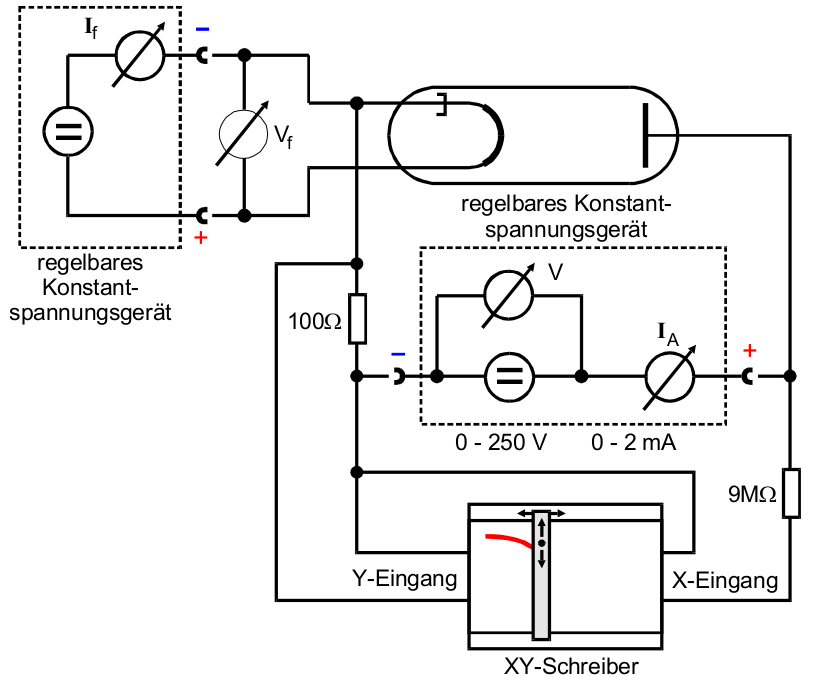
\includegraphics[height=7cm]{logos/Schaltung-Diodenkennlinie.png}
  \caption{Schaltung zur Messung der Diodenkennlinien \cite{Anleitung}.}
  \label{fig:SDL}
\end{figure}
Zur Messung des Anlaufstroms wird der Versuchsaufbau wie in der Darstellung \ref{fig:SAK} aufgebaut.
Für die maximale Heizleistung wird nun die Spannung von 0 bis \SI{1}{\volt}
schrittweise erhöht und wieder die Stromstärke notiert.

\begin{figure}
  \centering
  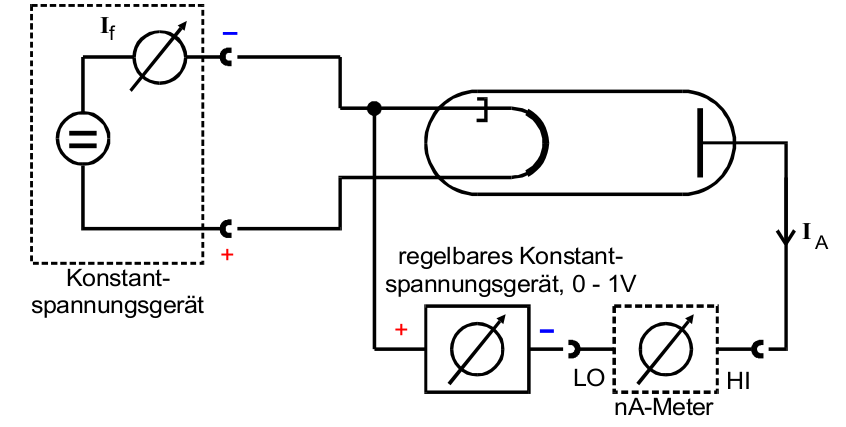
\includegraphics[height=3cm]{logos/Schaltung-Anlaufstromkurve.png}
  \caption{Schaltung zur Messung der Anlaufstromkurve \cite{Anleitung}.}
  \label{fig:SAK}
\end{figure}
